\documentclass[../main]{subfiles}

\begin{document}

\chapter{Results}
This chapter will discuss the results of the training, validation and testing.
In the first section the configurations with the best results will be shown with their average scores obtained during training and validation.
Subsequently, the results obtained from the best configurations will be shown in the testing section.
All f1-scores are accompanied by a defined interval thanks to the t-student, with an accuracy of 90\%.

\section{Validation}
The hyperparameters of the configurations with the best validation results are shown in Tables \ref{table:sklearn_model_best_conf} and \ref{table:torch_model_best_conf}.
In particular, the hyper parameters that led the models to achieve the best results are shown.
\begin{table}[!ht]
    \center
    \begin{tabular}{|l|l|}
        \hline
        \multicolumn{1}{|c|}{\textbf{Model}} & \multicolumn{1}{c|}{\textbf{Best configuration}}                                                    \\
        \hline
        \textit{RandomForestClassifier}    & \begin{tabular}[c]{@{}l@{}}n\_estimators: 700\\ max\_features: 'sqrt'\\ max\_depth: 10\end{tabular} \\
        \hline
        \textit{DecisionTreeClassifier}    & \begin{tabular}[c]{@{}l@{}}criterion: 'gini'\\ max\_depth: 10\end{tabular}                      \\
        \hline
        \textit{GaussianNB}                & var\_smoothing: 1.873817422860383e-06                                                              \\
        \hline
        \textit{QDA}                       & \begin{tabular}[c]{@{}l@{}}reg\_param: 1e-3\\ tol: 1e-4\end{tabular}                            \\
        \hline % TODO: wait result
        \textit{SVM}                       & \begin{tabular}[c]{@{}l@{}}C: 100\\ gamma: 1e-2\\ kernel: 'rbf'\end{tabular}                       \\
        \hline
    \end{tabular}
    \caption{Best configurations for scikit-learn models.}
    \label{table:sklearn_model_best_conf}
\end{table}

\begin{table}[!ht]
    \center
    \begin{tabular}{|l|l|}
        \hline
        \multicolumn{1}{|c|}{\textbf{Model}} & \multicolumn{1}{c|}{\textbf{Best configuration}}                                                                                                                  \\
        \hline
        \textit{MovieNet (MLP)}     & \begin{tabular}[c]{@{}l@{}}n\_hidden\_layers: 3\\ dropout: 0.2\\ batch\_norm: False\\ batch\_size: 128\\ optim: optimizer.Adam\\ weight\_decay: 1e-7\end{tabular} \\
        \hline
    \end{tabular}
    \caption{Best configuration for PyTorch model.}
    \label{table:torch_model_best_conf}
\end{table}
\newpage

From the best configuration of MovieNet, some observations can be made:
\begin{itemize}
    \item In general, the best configurations have a number of hidden layers equal to the smallest value defined in the range.
    \item The value of weight decay was the smallest in the range, probably because the network was able to generalize the problem without overfitting.
\end{itemize}
The scikit-learn models will be commented on directly afterwards, so that the results can be compared.
The f1-score obtained by each model during the training and validation phase is shown in the Table \ref{table:train_val_results}.


\begin{table}[!ht]
    \center
    \begin{tabular}{|l|cc|}
        \hline
        \multicolumn{1}{|c|}{\multirow{2}{*}{\textbf{Model}}} & \multicolumn{1}{c|}{\textbf{Training}} & \multicolumn{1}{l|}{\textbf{Validation}} \\
        \cline{2-3} 
        \multicolumn{1}{|c|}{}                                & \multicolumn{2}{c|}{\textbf{f1-score (\%)}}                                       \\
        \hline
        \textit{RandomForestClassifier}                       & \multicolumn{1}{c|}{96.3 $\pm$0.1}         & 75.5 $\pm$0.1                               \\
        \hline
        \textit{DecisionTreeClassifier}                       & \multicolumn{1}{c|}{79.4 $\pm$0.4}        & 66 $\pm$0.8                                \\
        \hline
        \textit{GaussianNB}                                   & \multicolumn{1}{c|}{51 $\pm$0.3}         & 45 $\pm$0.2                                \\
        \hline
        \textit{QDA}                                          & \multicolumn{1}{c|}{97 $\pm$0.06}        & 49.6 $\pm$0.3                               \\
        \hline %TODO: wait result
        \textit{SVM}                                          & \multicolumn{1}{c|}{99.9 $\pm$0.001}       & 96.1 $\pm$0.09                               \\
        \hline
        \textit{MovieNet (MLP)}                               & \multicolumn{1}{c|}{87.5 $\pm$0.1}         & 79.5 $\pm$0.08                               \\
        \hline
    \end{tabular}
    \caption{Training and validation results of each model with the best configurations.}
    \label{table:train_val_results}
\end{table}

\begin{figure}[!ht]
    \center
    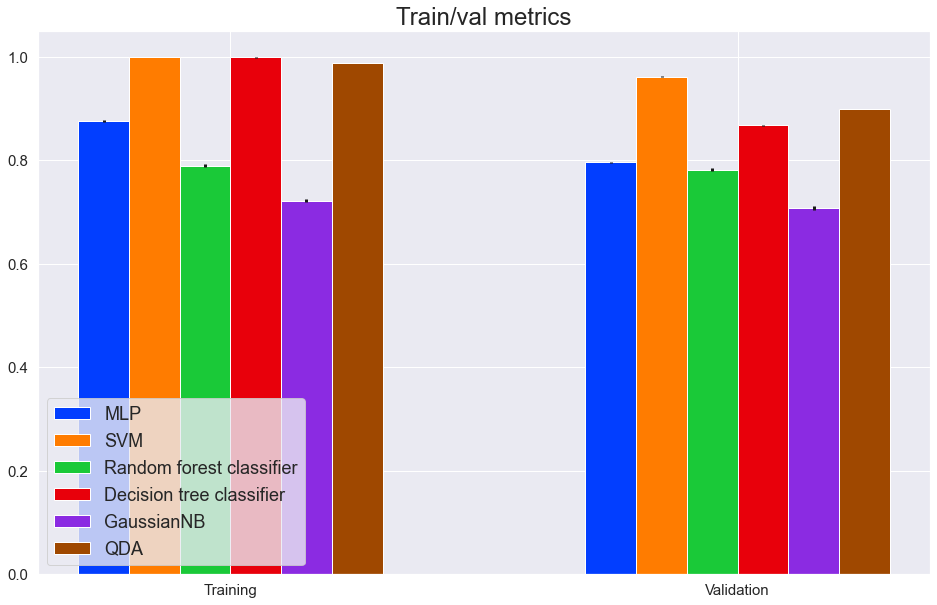
\includegraphics[width=0.8\linewidth]{figures/train_val_plot.png}
    \caption{Multiplebar plot that shows the train/val f1-score for each model.}
    \label{fig:train_val_plot}
\end{figure}
\newpage

It can be seen that SVM managed to achieve a higher f1 score in both training and validation.

\section{Testing}
The test phase is necessary to evaluate the performance of the model using samples that have never been taken.
It can be seen in Table \ref{table:test_results} how SVM and MovieNet achieved the highest metrics with the lowest losses.
Instead, probabilistic models are the ones that have obtained worse metrics.

\begin{table}[!ht]
    \center
    \begin{tabular}{|l|cc|}
        \hline
        \multicolumn{1}{|c|}{\multirow{2}{*}{\textbf{Model}}} & \multicolumn{2}{c|}{\textbf{Testing}}               \\
        \cline{2-3} 
        \multicolumn{1}{|c|}{}                                & \multicolumn{1}{c|}{\textbf{f1-score (\%)}} & \textbf{loss}  \\ 
        \hline
        \textit{RandomForestClassifier}                       & \multicolumn{1}{c|}{75.7 $\pm$0.5}             & 0.242 \\
        \hline
        \textit{DecisionTreeClassifier}                       & \multicolumn{1}{c|}{65.3 $\pm$0.9}                & 0.348  \\
        \hline
        \textit{GaussianNB}                                   & \multicolumn{1}{c|}{7.4 $\pm$0.5}                & 0.837 \\
        \hline
        \textit{QDA}                                          & \multicolumn{1}{c|}{14.3 $\pm$0.004}              & 0.693 \\
        \hline % TODO: wait result
        \textit{SVM}                                          & \multicolumn{1}{c|}{82.8 $\pm$0.4}              & 0.17  \\
        \hline
        \textit{MovieNet (MLP)}                                     & \multicolumn{1}{c|}{85.9 $\pm$0.3}              & 0.36  \\ \hline
    \end{tabular}
    \caption{Testing results of each model with the best configurations.}
    \label{table:test_results}
\end{table}

\begin{figure}[!ht]
    \center
    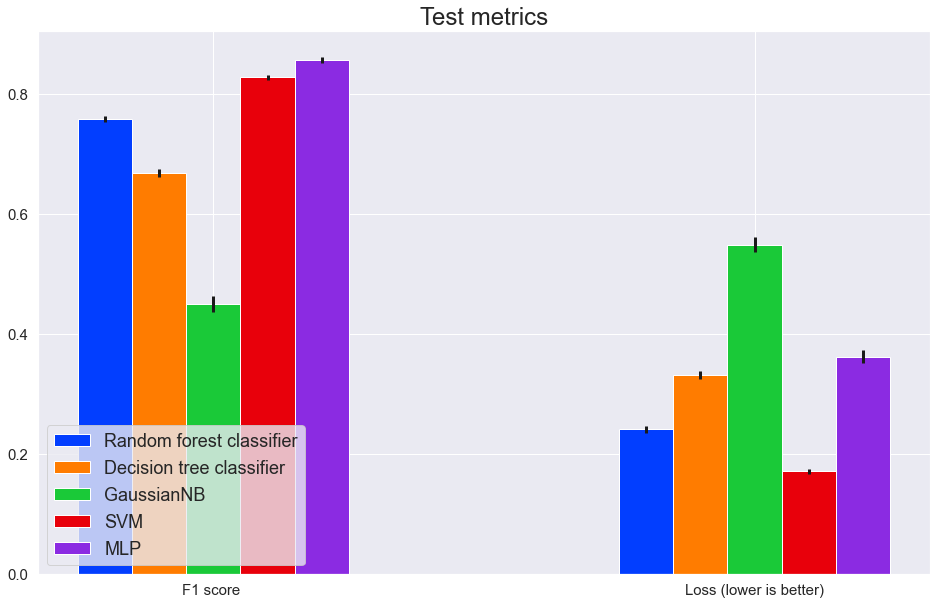
\includegraphics[width=0.8\linewidth]{figures/test_metric_plot.png}
    \caption{Multiplebar plot that shows the test f1-score for each model.}
    \label{fig:test_metric_plot}
\end{figure}
\newpage

The reasons why the test results on the tree-based and naive bayes models are low could be related to the unbalance of the dataset as the test set contains the initial distribution of classes.
The use of different test sets following cross validation did not affect the performance of the models.
In fact, the confidence intervals are quite small, which means that the models were able to predict in the same way regardless of the test set.

\end{document}